\section{Results and Factory Case Studies}
\label{sec:results}
\begin{table*}[!t]\begin{adjustwidth}{-\extralength}{0cm}\centering
\caption{Corpus and original transcript diagnostics. Activity and process columns show permitted/used labels. Coverage uses unions divided by parsed endpoint spans, not verified video duration. Alignment is boundary agreement within five seconds under the original parser.}
\label{tab:corpus}\small\setlength{\tabcolsep}{4pt}
\begin{tabular}{@{}lrrrrrrr@{}}\toprule
Factory & Workers & Videos & Events & Activities & Processes & Coverage & Alignment \\\midrule
\textbf{001} & 11 & 97 & 2{,}288 & 131/125 & 13/13 & 94.8\% & 93.1\% \\
\textbf{002} & 10 & 54 & 1{,}541 & 75/67 & 24/24 & 28.2\% & 71.8\% \\
\textbf{003} & 11 & 72 & 2{,}449 & 55/52 & 12/12 & 93.0\% & 86.8\% \\
\textbf{004} & 10 & 51 & 1{,}893 & 71/65 & 22/22 & 92.1\% & 90.4\% \\
\textbf{005} & 11 & 22 & 1{,}103 & 102/97 & 18/17 & 25.0\% & 75.0\% \\
\textbf{006} & 6 & 26 & 1{,}424 & 61/59 & 24/24 & 14.1\% & 62.1\% \\\midrule
All & 59 & 322 & 10{,}698 & & & 52.8\% & 82.1\% \\
\bottomrule\end{tabular}\end{adjustwidth}\end{table*}

\subsection{\textbf{RQ1}: Construction and structural properties}
\label{sec:structure}
Table~\ref{tab:corpus} reports the released corpus. All 10{,}698 events have the required values, nonnegative ordered endpoints, and labels in the relevant factory lists. Start times are nondecreasing within each log. There are no empty logs or zero-duration events. However, 35 adjacent event pairs overlap, 20 in factory \textbf{001} and 15 in factory \textbf{002}. Passing schema and vocabulary checks therefore does not imply a non-overlapping segmentation. Activity vocabulary use ranges from 89.3\% to 96.7\%.

\subsection{\textbf{RQ2}: Consistency with generated transcripts}
\label{sec:consistency}
The original parser finds 82.1\% of event boundaries within five seconds of a recognized transcript endpoint. It yields an overall coverage diagnostic of 52.8\%. Neither statistic is video accuracy. The coverage denominator is heavily affected by the literal multi-hour endpoints listed in Table~\ref{tab:anomalies}. Alignment can also be low when formats change or when S4 splits a narrated interval. These diagnostics alone do not establish extraction truncation.

\begin{table*}[!t]\begin{adjustwidth}{-\extralength}{0cm}\centering
\caption{Author judgments of event support and transcript-entry overlap against generated transcripts.}
\label{tab:audit}\small
\begin{tabularx}{\linewidth}{@{}l r L@{}}\toprule
Sample outcome & Count & Interpretation \\\midrule
Event fully supported (C) & 36 & Strict transcript support: 36/42, or 85.7\% \\
Event partially supported (P) & 6 & Context is plausible; overlapping description is insufficient \\
Event contradicted (X) & 0 & No contradiction among the sampled events \\
Transcript entry overlaps (COV) & 34 & At least one event overlaps; action completeness not established \\
Uncovered, non-operational (EXC) & 4 & Excluded from the archive's reported overlap denominator \\
Uncovered, operational (MISS) & 4 & Reported entry-overlap rate: 34/38, or 89.5\% \\
\bottomrule\end{tabularx}\end{adjustwidth}\end{table*}

Table~\ref{tab:audit} summarizes the archived judgments. Partial-support examples show the difficulty of checking events against compressed text. Event sample 5 assigns a particular bagging activity where the transcript only states that repetitive assembly and packaging continue. Sample 40 assigns guiding an upper mold half where the text only says that the worker helps with a mold. Recall sample 10 uses a transcript interval from 11:51:00 to 12:59:00 in an anomalous file whose event log ends at 00:20:00. Its MISS judgment is preserved, but the original explanation as long-recording truncation is unverified. These cases show why a single accuracy label would obscure different sources of uncertainty.

\subsection{An end-to-end foundry example}
\label{sec:worked}
Consider factory \textbf{006}, worker 003, recording 00003. The S1 transcript interval from 00:04:05 to 00:04:36 describes placing an empty frame on a pattern plate, pouring and hand-packing powder, and using a wooden tool to level the surface. The S2 summary describes preparation, filling, packing, leveling, and compression of molds. It compresses many recordings into a worker-level account. The S3 report supplies process \emph{Sand mold creation}, activity \emph{level powder surface with wooden scraper}, and a compact summary of this worker's molding work.

\begin{figure*}[!t]\begin{adjustwidth}{-\extralength}{0cm}\centering
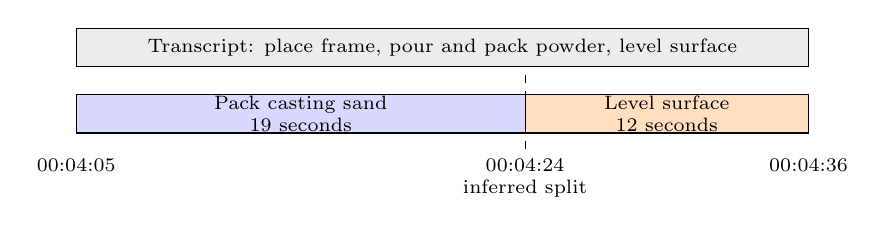
\begin{tikzpicture}[x=0.30cm,y=0.7cm,font=\small]
\draw[fill=gray!15] (0,2) rectangle (31,2.7);
\node[align=center,font=\scriptsize] at (15.5,2.35){Transcript: place frame, pour and pack powder, level surface};
\draw[fill=blue!15] (0,0.8) rectangle (19,1.5);
\draw[fill=orange!25] (19,0.8) rectangle (31,1.5);
\node[font=\scriptsize,align=center] at (9.5,1.15){Pack casting sand\\19 seconds};
\node[font=\scriptsize,align=center] at (25,1.15){Level surface\\12 seconds};
\draw[dashed] (19,0.5)--(19,1.9);
\node[below,font=\scriptsize] at (0,0.5){00:04:05};
\node[below,font=\scriptsize,align=center] at (19,0.5){00:04:24\\inferred split};
\node[below,font=\scriptsize] at (31,0.5){00:04:36};
\end{tikzpicture}
\caption{Exact transcript and event intervals for the foundry example. The original transcript is line 16 of its text file; the events are data rows 17 and 18 of the corresponding CSV. Bar lengths show recorded durations, not independently checked action boundaries.}
\label{fig:worked}\end{adjustwidth}\end{figure*}

S4 produces two events within that 31-second transcript interval: \emph{pack casting sand into mold frame}, from 00:04:05 to 00:04:24, and \emph{level powder surface with wooden scraper}, from 00:04:24 to 00:04:36. Both have process \emph{Sand mold creation}. Figure~\ref{fig:worked} shows what is retained and added. The internal boundary at 00:04:24 is inferred; S1 does not timestamp that transition separately. The events compress placement, pouring, and joint hand-packing into the first activity and add controlled names and a process context.

\begin{lstlisting}[caption={Illustrative JSON reconstructed from CSV data row 18. It is not an archived model response.},label={lst:reconstructed}]
{"events": [{
  "estimated_start_time": "00:04:24",
  "estimated_end_time": "00:04:36",
  "activity": "level powder surface with wooden scraper",
  "process": "Sand mold creation"
}]}
\end{lstlisting}

The linked transcript, worker summary, factory report, and event log preserve the successive representations of this recording. S5 retains the recording identifier and local offsets alongside shifted timestamps. Audit event 41 judges the leveling event fully supported by its transcript. This supports the label's textual basis, not the exact internal split or a video-based duration measurement.

\subsection{\textbf{RQ3}: Descriptive analytical capabilities}
\label{sec:analyses}
\subsubsection{Time composition and category transitions}
\begin{table*}[!t]\begin{adjustwidth}{-\extralength}{0cm}\centering
\caption{Reproduced time analysis on 320 logs. Left: percentage of summed event duration. Right: factory medians over eligible workers, after the original worker-level rounding. A run sums consecutive same-category rows within a clip; transition counting can cross clips.}
\label{tab:value}\footnotesize\setlength{\tabcolsep}{3pt}
\begin{tabular}{@{}lrrrrrrr rrr@{}}\toprule
 & \multicolumn{7}{c}{Process-based category shares (\%)} & \multicolumn{3}{c}{Worker summaries}\\
\cmidrule(lr){2-8}\cmidrule(l){9-11}
Factory & VA & MH & TR & QI & CM & RW & DOC & VA (\%) & Trans./h & Mean run (min) \\\midrule
\textbf{001} & 93.1 & 4.1 & 1.8 & 0.0 & 0.2 & 0.0 & 0.9 & 94.5 & 9.2 & 4.6 \\
\textbf{002} & 96.3 & 0.1 & 2.3 & 0.2 & 0.0 & 0.0 & 1.1 & 97.3 & 3.9 & 8.8 \\
\textbf{003} & 82.1 & 0.4 & 0.0 & 0.0 & 6.3 & 10.8 & 0.4 & 86.4 & 3.6 & 9.0 \\
\textbf{004} & 89.9 & 3.0 & 3.5 & 2.0 & 0.9 & 0.0 & 0.7 & 91.3 & 10.6 & 3.6 \\
\textbf{005} & 80.6 & 5.4 & 9.7 & 4.3 & 0.0 & 0.0 & 0.0 & 85.9 & 5.6 & 6.2 \\
\textbf{006} & 74.2 & 12.1 & 7.8 & 0.0 & 5.7 & 0.0 & 0.3 & 87.0 & 14.4 & 3.1 \\
\bottomrule\end{tabular}\end{adjustwidth}\end{table*}

\FloatBarrier
Table~\ref{tab:value} reproduces the existing category shares using the actual two-log exclusion rule. The non-VA category share ranges from 3.7\% to 25.8\% of retained summed event duration. This is neither total worker time nor recoverable capacity. Factory \textbf{003} assigns 10.8\% to defect patching. Its factory report already describes defect patching in the opening overview and vocabulary. The duration share quantifies this recorded behavior under an explicit category rule.

\begin{figure*}[!t]\begin{adjustwidth}{-\extralength}{0cm}\centering
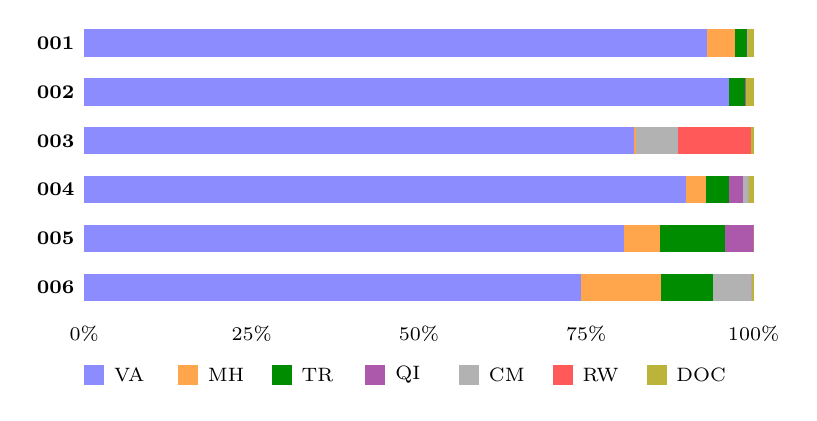
\begin{tikzpicture}[x=0.085cm,y=0.62cm,font=\scriptsize]
\node[left] at (0,0){\textbf{001}};
\fill[blue!45] (0,-0.28) rectangle (93.05718144979738,0.28);
\fill[orange!70] (93.05718144979738,-0.28) rectangle (97.14092751013057,0.28);
\fill[green!55!black] (97.14092751013057,-0.28) rectangle (98.93561458802341,0.28);
\fill[violet!65] (98.93561458802341,-0.28) rectangle (98.93561458802341,0.28);
\fill[gray!60] (98.93561458802341,-0.28) rectangle (99.09230076542099,0.28);
\fill[red!65] (99.09230076542099,-0.28) rectangle (99.09230076542099,0.28);
\fill[yellow!70!black] (99.09230076542099,-0.28) rectangle (100.0,0.28);
\node[left] at (0,-1){\textbf{002}};
\fill[blue!45] (0,-1.28) rectangle (96.33507853403141,-0.72);
\fill[orange!70] (96.33507853403141,-1.28) rectangle (96.38647094722641,-0.72);
\fill[green!55!black] (96.38647094722641,-1.28) rectangle (98.69591751517682,-0.72);
\fill[violet!65] (98.69591751517682,-1.28) rectangle (98.87097292262229,-0.72);
\fill[gray!60] (98.87097292262229,-1.28) rectangle (98.87097292262229,-0.72);
\fill[red!65] (98.87097292262229,-1.28) rectangle (98.87097292262229,-0.72);
\fill[yellow!70!black] (98.87097292262229,-1.28) rectangle (99.99999999999999,-0.72);
\node[left] at (0,-2){\textbf{003}};
\fill[blue!45] (0,-2.2800000000000002) rectangle (82.07314107241146,-1.72);
\fill[orange!70] (82.07314107241146,-2.2800000000000002) rectangle (82.46995123075152,-1.72);
\fill[green!55!black] (82.46995123075152,-2.2800000000000002) rectangle (82.46995123075152,-1.72);
\fill[violet!65] (82.46995123075152,-2.2800000000000002) rectangle (82.46995123075152,-1.72);
\fill[gray!60] (82.46995123075152,-2.2800000000000002) rectangle (88.75107202744391,-1.72);
\fill[red!65] (88.75107202744391,-2.2800000000000002) rectangle (99.55710866198176,-1.72);
\fill[yellow!70!black] (99.55710866198176,-2.2800000000000002) rectangle (100.00000000000001,-1.72);
\node[left] at (0,-3){\textbf{004}};
\fill[blue!45] (0,-3.2800000000000002) rectangle (89.85731229558279,-2.7199999999999998);
\fill[orange!70] (89.85731229558279,-3.2800000000000002) rectangle (92.89436796894655,-2.7199999999999998);
\fill[green!55!black] (92.89436796894655,-3.2800000000000002) rectangle (96.39327175358517,-2.7199999999999998);
\fill[violet!65] (96.39327175358517,-3.2800000000000002) rectangle (98.3592711066384,-2.7199999999999998);
\fill[gray!60] (98.3592711066384,-3.2800000000000002) rectangle (99.30453222154334,-2.7199999999999998);
\fill[red!65] (99.30453222154334,-3.2800000000000002) rectangle (99.30453222154334,-2.7199999999999998);
\fill[yellow!70!black] (99.30453222154334,-3.2800000000000002) rectangle (100.00000000000001,-2.7199999999999998);
\node[left] at (0,-4){\textbf{005}};
\fill[blue!45] (0,-4.28) rectangle (80.58529621698787,-3.7199999999999998);
\fill[orange!70] (80.58529621698787,-4.28) rectangle (85.9880305276451,-3.7199999999999998);
\fill[green!55!black] (85.9880305276451,-4.28) rectangle (95.71185417009829,-3.7199999999999998);
\fill[violet!65] (95.71185417009829,-4.28) rectangle (100.00000000000001,-3.7199999999999998);
\fill[gray!60] (100.00000000000001,-4.28) rectangle (100.00000000000001,-3.7199999999999998);
\fill[red!65] (100.00000000000001,-4.28) rectangle (100.00000000000001,-3.7199999999999998);
\fill[yellow!70!black] (100.00000000000001,-4.28) rectangle (100.00000000000001,-3.7199999999999998);
\node[left] at (0,-5){\textbf{006}};
\fill[blue!45] (0,-5.28) rectangle (74.15951726119617,-4.72);
\fill[orange!70] (74.15951726119617,-5.28) rectangle (86.22388243503961,-4.72);
\fill[green!55!black] (86.22388243503961,-5.28) rectangle (93.97397479578014,-4.72);
\fill[violet!65] (93.97397479578014,-5.28) rectangle (93.97397479578014,-4.72);
\fill[gray!60] (93.97397479578014,-5.28) rectangle (99.71265547391322,-4.72);
\fill[red!65] (99.71265547391322,-5.28) rectangle (99.71265547391322,-4.72);
\fill[yellow!70!black] (99.71265547391322,-5.28) rectangle (100.0,-4.72);
\node[below] at (0,-5.6){0\%};
\node[below] at (25,-5.6){25\%};
\node[below] at (50,-5.6){50\%};
\node[below] at (75,-5.6){75\%};
\node[below] at (100,-5.6){100\%};
\fill[blue!45] (0,-7) rectangle (3,-6.6);
\node[right] at (3,-6.8){VA};
\fill[orange!70] (14,-7) rectangle (17,-6.6);
\node[right] at (17,-6.8){MH};
\fill[green!55!black] (28,-7) rectangle (31,-6.6);
\node[right] at (31,-6.8){TR};
\fill[violet!65] (42,-7) rectangle (45,-6.6);
\node[right] at (45,-6.8){QI};
\fill[gray!60] (56,-7) rectangle (59,-6.6);
\node[right] at (59,-6.8){CM};
\fill[red!65] (70,-7) rectangle (73,-6.6);
\node[right] at (73,-6.8){RW};
\fill[yellow!70!black] (84,-7) rectangle (87,-6.6);
\node[right] at (87,-6.8){DOC};
\end{tikzpicture}

\caption{Category composition calculated from retained event rows and the released process map. Segments use unrounded duration totals; Table~\ref{tab:value} reports rounded percentages. Factories have different task mixes and label schemes, so the plot does not rank efficiency.}
\label{fig:composition}\end{adjustwidth}\end{figure*}

Figure~\ref{fig:composition} displays the category shares. The mean-run column is the median across workers of their \emph{mean} VA-run durations. A value of 3.1 minutes in factory \textbf{006} is a central tendency; it says nothing about the longest VA episode. Factory \textbf{001} has 449 MH/TR rows, a mean row duration of 14.54 seconds, and 14.6 such rows per summed event-hour. Factory \textbf{006} has 192 MH/TR rows, a mean of 25.14 seconds, and 28.4 rows per summed event-hour. These are row-based descriptions. Segmentation, repeated-action compression, and clip joins influence their values.

\subsubsection{Process flow and discovery}
\label{sec:discovery}
Video-as-case traces describe observation windows. Among the 97, 54, 72, 51, 22, and 26 videos in factories \textbf{001} to \textbf{006}, there are respectively 97, 53, 70, 51, 22, and 26 distinct activity traces. Self-loops account for 4.3\% to 16.8\% of within-video directly-follows pairs. These statistics are reproduced directly from the stored labels. A self-loop can reflect separately extracted repetitions or segmentation choices; it is not a count of manufactured items.

The released discovery script uses Inductive Miner~\cite{leemans2013inductive} with noise threshold 0.2, video cases, and activity labels. Appendix~\ref{supp-app:discovery} of the Additional Material records the repeated calculation and current dependency version. The recalculated fitness ranges from 0.9544 to 0.9910 and precision from 0.0603 to 0.2679. Fitness measures how the discovered model can replay the inferred traces; precision measures how much additional behavior it permits relative to that log. Both are properties of a model-log pair, not accuracy against actual factory behavior.

Many distinct traces and low precision can arise from flexible work, recording boundaries, abstraction choices, label variation, or extraction mistakes. The present evidence does not separate these causes. No process-level discovery result is reported because its computation and saved output are unavailable. Replacing activity labels with process labels would change the represented behavior and evaluation target. A higher precision after that change would not by itself be a controlled demonstration of better extraction or modeling.

\subsubsection{Worker profiles and shared dominant processes}
\label{sec:workers}
\begin{table*}[!t]\begin{adjustwidth}{-\extralength}{0cm}\centering
\caption{Selected shared-dominant-process groups, using the original eligibility and rounding rules. Ranges summarize worker profiles; they are not estimates of individual efficiency.}
\label{tab:bench}\footnotesize
\begin{tabularx}{\linewidth}{@{}lLrll@{}}\toprule
Factory & Dominant process & Workers & VA share & Mean VA run \\\midrule
\textbf{001} & Manual mechanical assembly & 6 & 89.7 to 97.8\% & 1.7 to 6.7 min \\
\textbf{001} & Metal stamping & 3 & 90.6 to 98.5\% & 3.2 to 7.9 min \\
\textbf{003} & Surface finishing and polishing & 5 & 67.3 to 96.9\% & 3.3 to 13.7 min \\
\textbf{004} & Garment ironing & 2 & 52.8 to 77.1\% & 3.5 to 4.1 min \\
\textbf{004} & Overlock seaming & 4 & 87.8 to 96.5\% & 1.5 to 10.3 min \\
\textbf{005} & Manual lathe machining & 2 & 95.0 to 95.8\% & 6.9 to 9.4 min \\
\bottomrule\end{tabularx}\end{adjustwidth}\end{table*}

\FloatBarrier
A shared vocabulary permits descriptive comparison within a factory. Table~\ref{tab:bench} groups workers by their largest process-duration total, then compares VA shares over \emph{all} retained events for those workers. Eligibility requires at least 1{,}800 seconds of summed event duration. It does not require verified footage duration or equivalent tasks. There are 11, 10, 10, 10, 5, and 5 eligible workers in factories \textbf{001} to \textbf{006}.

The 29.6 percentage-point range in the surface-finishing group describes different observed profiles. Differences may reflect task mix, product requirements, recording selection, category assignment, or working conditions. Likewise, the small range for two lathe workers cannot rule out differences in behavior. Neither result supports individual performance rankings.

\subsection{Six descriptive factory cases}
\label{sec:factorycases}
Each case below states its recorded scope, quantitative result, relationship to the report, and unresolved interpretation. Factory descriptions are derived from the reports. Cross-factory rankings are limited by different vocabularies, products, and observation windows.

\paragraph{Factory \textbf{001}: hardware stamping and assembly.}
The archive has 97 clips from 11 workers; the time analysis retains 95 clips. Manual mechanical assembly accounts for 55.7\% of retained summed duration, metal stamping for 18.2\%, and component bagging for 11.3\%. The report already describes material replenishment, floor storage, and operator transport. The 449 MH/TR rows and their short mean duration quantify the assigned category pattern. They motivate examining material presentation, but do not establish that dedicated handlers, shorter travel, or a different layout would improve output. Product mix and compressed repetitions remain competing explanations.

\paragraph{Factory \textbf{002}: garment finishing and packaging.}
There are 54 clips from ten workers, all retained by the event-end rule. Fabric folding, garment bagging, and ironing contribute 18.8\%, 17.1\%, and 13.2\% of summed duration. VA is 96.3\%. The report already describes transport, floor staging, and varied folding methods. Quantification shows a small separately categorized handling and transport share, not proof that those behaviors are rare within other processes. Two anomalous transcript endpoints and mixed formats weaken temporal interpretation. Product-specific finishing requirements and category boundaries need examination before any claim of superior efficiency.

\paragraph{Factory \textbf{003}: surface preparation and assembly.}
The archive covers 72 clips from 11 workers; all clips are retained. Surface finishing and polishing contributes 42.1\%, wax pattern assembly 19.2\%, and defect patching 10.8\%. The report already identifies patching and material transport. The log quantifies patching's share without establishing defect rates, avoidable rework, or financial loss. It also records 101 transport events totaling 1{,}230 seconds even though the process-based TR share is zero. This case demonstrates how aggregation can hide an extracted behavior. Material types and quality criteria remain uncertain in the report itself.

\paragraph{Factory \textbf{004}: garment sewing and finishing.}
There are 51 clips from ten workers, all retained. Overlock seaming contributes 23.5\%, garment folding 11.0\%, and thread trimming 10.8\%. The median worker VA-transition rate is 10.6 per summed event-hour. The report already describes tool switching, material handling, and inspection. The logs add a reproducible category pattern and a 24.3 percentage-point VA-share range in the two-worker ironing group. Product specifications, additional finishing duties, and recording windows could explain this difference. The data do not identify which changes to tools or stations would help.

\paragraph{Factory \textbf{005}: machining and motor assembly.}
The archive contains 22 clips from 11 workers, with only five workers meeting the time threshold. All clips are retained. Manual lathe machining contributes 32.1\%, drill press machining 19.1\%, and material transport and logistics 9.7\%. The report describes staging, fixturing, inspection, and coupled workstations. The log adds duration shares, including 4.3\% assigned to dimensional inspection. The two lathe profiles have similar VA shares, but their task equivalence is unknown. Inspection can be necessary, and one transcript has an unresolved endpoint anomaly. The recorded shares cannot measure excess quality work or recoverable machine capacity.

\paragraph{Factory \textbf{006}: molding and foundry work.}
There are 26 clips from six workers, all retained; five workers meet the time threshold. Sand mold creation, pattern cleaning and coating, and compression molding contribute 17.4\%, 14.0\%, and 12.2\%. The report already describes floor staging, material movement, cleaning, and mold-track operations. The logs assign 19.8\% of summed duration to MH/TR and yield a median worker mean VA run of 3.1 minutes. These quantities support a closer study of handling requirements, not a diagnosis of layout as their cause. Necessary mold preparation, differing materials, and segmentation choices are alternatives. Two transcript endpoints require resolution against source metadata.

\begin{table*}[!t]\begin{adjustwidth}{-\extralength}{0cm}
\caption{Evidence-linked hypotheses. These are candidates for investigation; intervention effects were not measured.}
\label{tab:hypotheses}\footnotesize
\begin{tabularx}{\linewidth}{@{}LLLL@{}}\toprule
Observation & Plausible explanation & Competing explanation & Evidence needed \\\midrule
\textbf{001}: 449 short MH/TR rows; 5.9\% of summed duration & Material presentation creates frequent replenishment & Segmentation splits one handling episode into several rows; task mix differs & Video checks, supply distances, batch quantities, station observations \\
\textbf{006}: 19.8\% MH/TR; frequent category transitions & Layout or replenishment arrangements require repeated movement & Heavy or fragile materials require necessary support work & Routes, loads, safety requirements, matched task observations \\
\textbf{003}: 10.8\% defect patching & Upstream defects require corrective work & Patching is a planned finishing requirement & Product specifications, defect criteria, item counts, upstream records \\
\textbf{003} and \textbf{004}: VA shares differ within dominant-process groups & Conditions or work allocation differ & Product mix, selection, or extraction differences & Comparable products and observation windows; independent video review \\
\textbf{005}: two similar lathe VA shares & Common station requirements shape profiles & Similar aggregate shares hide different tasks or behavior & Task-level comparisons and production context \\
\bottomrule\end{tabularx}\end{adjustwidth}\end{table*}

\FloatBarrier
\subsection{From observations to operational hypotheses}
Table~\ref{tab:hypotheses} connects observations to explanations and the evidence needed to distinguish them. Reports identify phenomena; logs can quantify them under a chosen representation. Explaining their causes requires additional evidence. Transport, inspection, cleaning, and documentation are not automatically waste, and the time assigned to them is not automatically available for production. No intervention effect or cost saving is demonstrated by these descriptive results.
